%\documentclass[numbers=noenddot, 12pt, a4paper, oneside]{scrbook}%
\documentclass[12pt, a4paper]{report}
\usepackage{blindtext}
\usepackage{fullpage}
\usepackage[utf8]{inputenc}
\usepackage{float}
\usepackage{hyperref}
\usepackage{hyperref}
\usepackage{tabularx}
\usepackage{graphicx}
\def\Plus{\texttt{+}}
\usepackage{listings}
\usepackage{xcolor}

\begin{document}

\begin{titlepage}
	\centering
	\vspace{1cm}
	\vspace{1cm}

	{\scshape\Large Game Design Document\par}
	\vspace{0.1cm}
	\begin{figure}[H]
		\centering
		\includegraphics[width=0.5\textwidth]{images/Logo}
	\end{figure}
	\vspace{1cm}
	\vspace{3cm}
	{\Large\itshape by\par}
	{\Large\itshape Gianluigi Oliva\par}
	{\Large\itshape Filippo Ghinelli, Leonardo Febbo, Lucia Ferrari\par}
	\vspace{1.5cm}
	\vfill



	\vfill

	% Bottom of the page
	{\large \today\par}
\end{titlepage}

\newpage
\tableofcontents
\newpage

\chapter{Overview and General Idea}
\section*{Introduction}
Terrible malware infected Tommy’s computer and he cannot use it anymore. When everything seems to be lost, here it comes: the help from a little hero… a lone bit by the name of Bitty. Our hero must travel to the core of the computer, fix all the bugs caused by the malware along the way, and then destroy the malware. Start with the high-level applications, such as a browser, and go on to the operating system to solve various harder problems. Free the imprisoned programs and ask them to help you during your adventure!\\

\textit{Bit&Byte} is a 2D puzzle game with stealth, cooperative and platforming elements, designed for PC. The visual style is simple and cartoony.\\

\section*{Description}
The player must solve puzzles to reach the exit. The world is arranged in an upside-down pyramid structure, divided in several layers: from the top to the bottom there is the Software Application Layer, then the Operating System Layer and lastly the System Kernel Layer. Our hero’s story is set in the Software Application Level, where he will travel through partitions and meet his allies. Inside the partitions, Bitty must progress through different levels.

In addition to Bitty, the player will be able to control other programs after liberating them and utilize their unique skills. In each level there are enemies and sensors that will immediately trigger an alarm, so it is necessary not to be spotted. The player can only control one character at a time, so it is recommended to switch characters when all of them are safe.
Thus, the gameplay features platforming, puzzle, stealth and co-op elements.\\

To complete each level it is necessary to collect the key to open the exit and then reach the door with \textit{all} characters that are available.

\section*{Audience and Marketing}
\textit{Bit&Byte} is designed to appeal to all ages, starting from the cartoony and friendly graphics. The individual puzzles have a degree of complexity such that they are entertaining for casual and hardcore gamers alike.\\
The main competitors for this game are games like \textit{Thomas Was Alone} --- where cooperation between playable characters is a key element for gameplay --- or \textit{Fez} --- for its puzzle-focused gameplay.

\section*{Genre(s)}
Platform, Stealth, Puzzle
\section*{Platform(s)}
Windows 10, macOS
\section*{Mode(s)}
Single-player

\chapter{Game Mechanics and Gameplay}
The main mechanics of \textit{Bit&Byte} are the cooperation between characters, the use different level elements and avoiding Virus enemies, as well as using the characters’ skills to create combinations and different interactions within the level.

\section*{Basic skills}
These are the basic skills and mechanics for all characters that the player can control:
\begin{itemize}
	\item \textbf{Walk}: Basic horizontal movement.
	\item \textbf{Jump}: A move to evade obstacles and go from one platform to another. It is possible to slightly change direction while airborne.
	\item \textbf{Interact}: Certain objects, like terminals and levers, can be acted upon to make something happen within a level.
\end{itemize}

Level failure can be caused by:
\begin{itemize}
  \item passing through a sensor
  \item touching a Virus
	\item getting hit by a Virus
  \item being detected by a Resident Virus
	\item falling on spikes
\end{itemize}



\section*{Character’s skills}
Each character has a unique skill which can be used in different ways to solve a puzzle.
\begin{itemize}
	\item \textbf{Bitty}: The protagonist and starting character of the game, he can collect one bit at a time and fire it in the direction he’s facing. The bits can be used to get rid of Spywares and to activate switches.
	\item \textbf{Shieldy}: A program that can stun Viruses from behind. Her ability can be turned on and off and covers a circular area around her. A Virus will remain stunned as long as it remains within the area of effect, otherwise it will come to its senses after 5 seconds.
	\item \textbf{Zippy}: A program that can shrink and stretch her body to fit tight spaces or offer extra jumping height. She can also shrink her allies if they are near her.
	\item \textbf{Gimpy}: A program that can camouflage himself to avoid being seen from enemies but he is still tangible.
\end{itemize}

\section*{Viruses’ skills}
There are different Virus enemies in the game, each representing one type of real world computer virus.
\begin{itemize}
	\item \textbf{Resident}: It is a sentinel with a long field of vision. If it detects the player it triggers an alarm that leads to level failure. This Virus stands still, it is dangerous only if the player touches it or walks into its field of vision.
	\item \textbf{Trojan}: It protects a predefined area in a level. If it spots the player, it will charge towards them at high speed. If it misses, it will turn around and go back to its original position.
	\item \textbf{Spyware}: It hangs from the ceiling by a string of code. It is harmless until the player walks below it: it will then drop down incredibly fast and most certainly catch the player.
	\item \textbf{Worm}: Very large and heavy, impossible to move or neutralize. It sleeps and blocks the way, preventing progress through the level.
	\item \textbf{Infector}: The Infector spreads its digital plague on several surfaces of the level, making them lethal to the touch.
	\item \textbf{Keylogger}: It has mastered the art of copying any and all inputs from the player and will imitate the movement of a character.
\end{itemize}




\section*{Camera}
%Since the game is based on puzzle resolution, the player must always have a complete view of the map, so a static camera is used which always shows the entire level and it's positioned at a fixed distance.\\
%Each time the player finishes a level the camera will show the next level, after a small cutscene. The camera will not be static only during the tutorial phase, which consists of a sliding level in which the player will experience all the basic mechanics.

Since the game is based on the resolution of the puzzles, the camera shows a large portion of the environment so that most elements needed to solve the puzzles are visible. The camera is centered on the active character and will move smoothly if the character is switched.

\section*{Hazards}
Viruses are not the only thing that the player must avoid.
\begin{itemize}
  \item \textbf{Laser}: Lasers are generated by small emitters. Some lasers are stationary, others can be rotated by interacting with a terminal and others will rotate autonomously. 
  \item \textbf{Spikes}: Spikes are generally positioned at the bottom of pits. It is possible to place objects over them in order to jump past them.
\end{itemize}

\section*{Interactables}
\begin{itemize}
	\item \textbf{Buttons}: Some can be pressed once to activate something, while others need something tangible (objects, characters) on top of them in order to stay activated.
	\item \textbf{Blocks}: They possess some weight and they can be pushed around the level to climb to higher places or keep buttons presed.
	\item \textbf{Moving Platforms and elevators}: They carry whatever sits on them. Some move on their own from the start while others must be activated with the press of a button or a switch.
	\item \textbf{Barriers/Gates}: They make some areas inaccessible to the player. By activating a button or switch they can be removed.
	\item \textbf{Terminal}: They have an “on” state and an “off” state. Most notably, you can change the direction of a laser by using a terminal.
\end{itemize}

\section*{Controls}
The in-game movement, like most of the puzzles, is physics-based. The active character is indicated by a small red cursor over their head. The player can change the active character according to the skills required to advance through the level.


\chapter{Story and World}
\textit{Bit&Byte} takes place inside a PC belonging to a young boy named Tommy. The PC got infected by a terrible virus which has made it unusable and Tommy doesn’t know how to fix it. He is unaware that a single brave bit is going to help him, so he is thinking of wiping the disk clean. Thus, Bitty has little time to destroy the Viruses. He cannot save the world alone, so he must find other programs to help him. However, they have been captured by the Viruses and Bitty must find a way to free them first.\\
The world of \textit{Bit&Byte} is an upside-down pyramid structure, much like Dante’s Inferno, starting from the Software Application Layer, going through the Operating System Layer and reaching the core, the System Kernel Layer. These layers or zones are divided into levels with puzzles. When a level begins, a small cutscene will advance the plot.

\section*{Characters}
Each character has their own personality.
\begin{itemize}
\item \textbf{Bitty}: A small and determined bit of few words, he would rather listen than speak.
\item \textbf{Shieldy}: A program with a strong sense of justice. She has made it her duty to protect her allies with her shield.
\item \textbf{Zippy}: A timid and introverted program. She handles most problems by shrinking down and finding a way around them.
\item \textbf{Gimpy}: A crafty program with a sparkling personality. He keeps the morale high through entertaining visual trickery.
\end{itemize}

\chapter{Art Overview}
The visual style for the environment is simple and linear and allows the player to imagine being inside a computer.
The playable characters are pill-shaped, with stubby limbs and cutesy button-like eyes. Bitty, Zippy and Gimpy have marks and features on their bodies which evoke their abilities. Shieldy and Gimpy carry their signature items with them, as a reminder to the player of what they can do.\\
The Viruses' bodies are more menacing, starting from their angry-looking eyes, sharper edges and more complex shapes.\\

\section*{Sketch and Characters Design}
\begin{figure}[H]
	\centering
	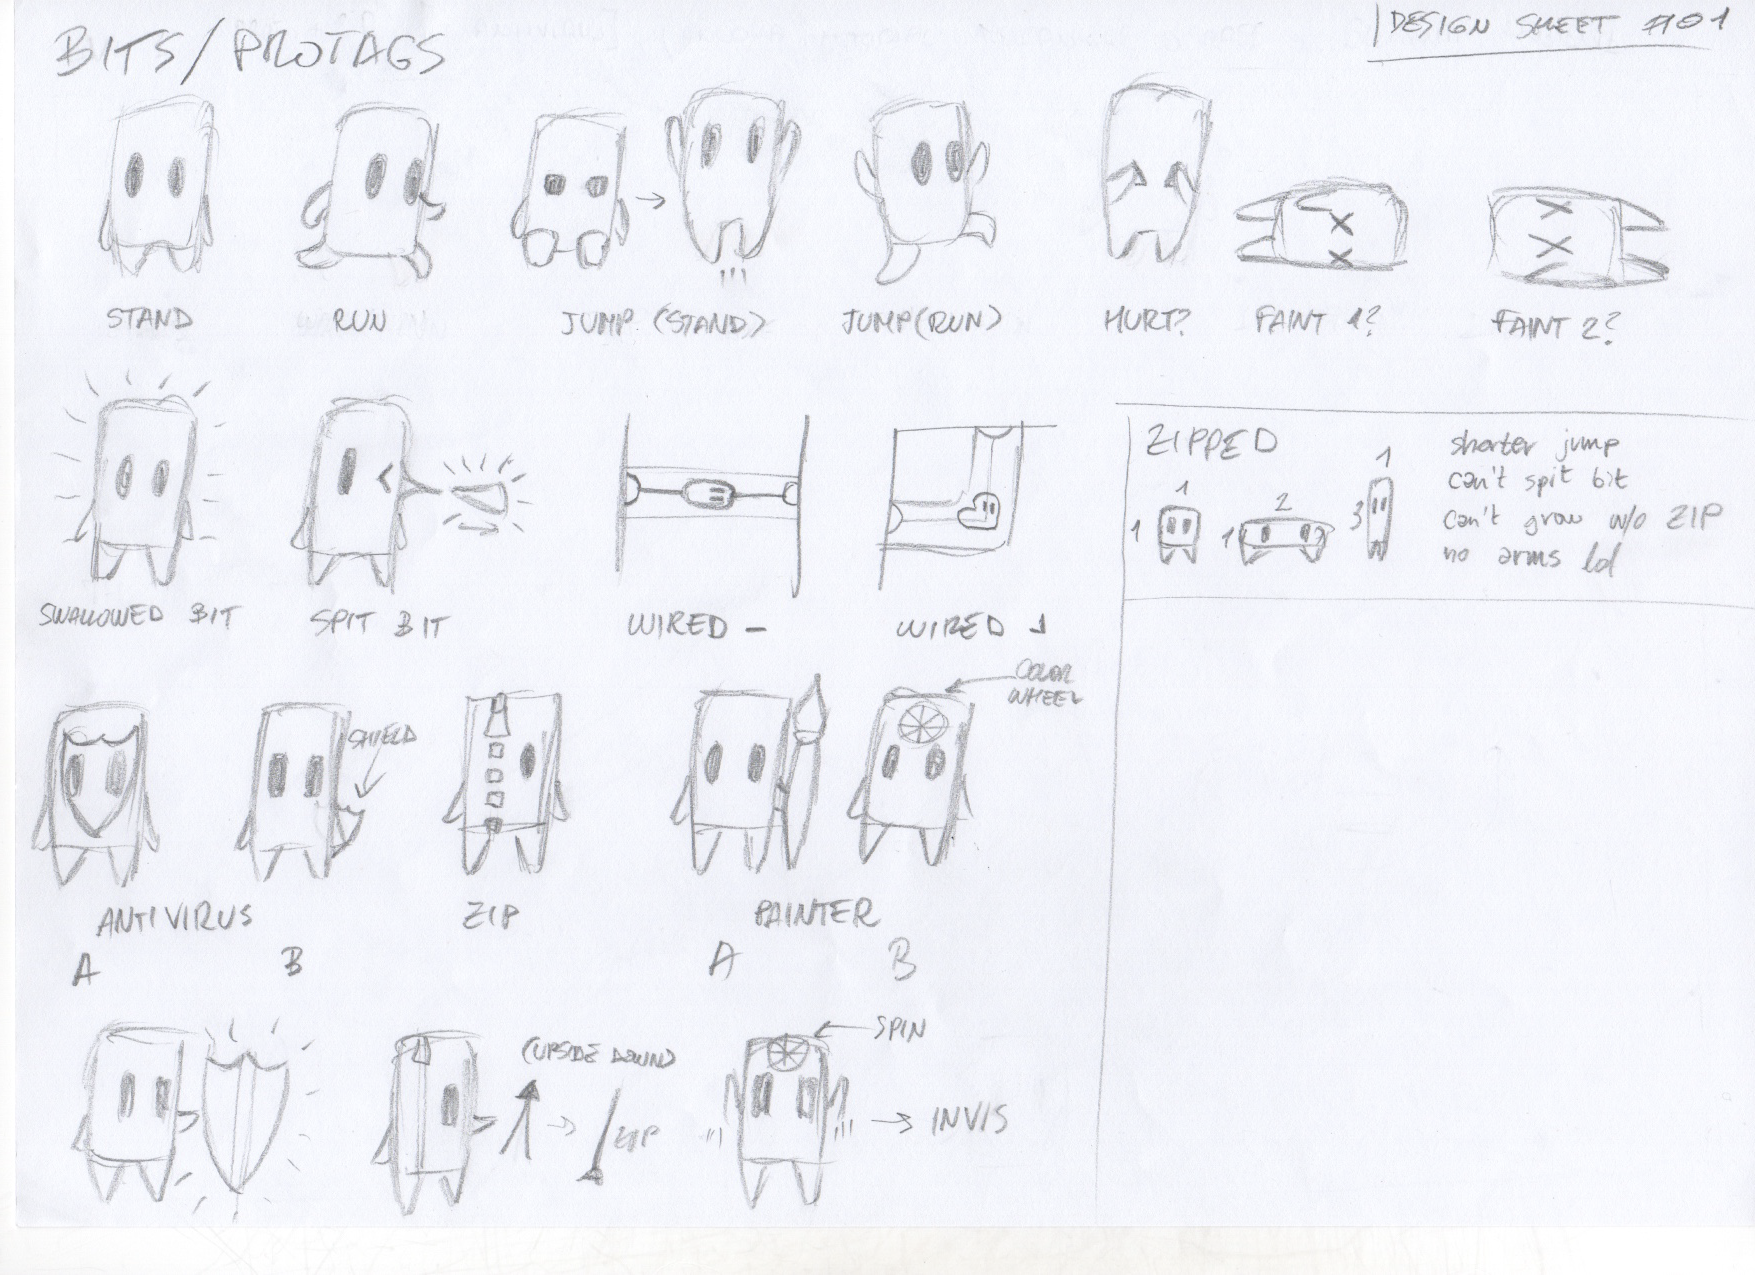
\includegraphics[width=0.5\textwidth]{images/Characters}
\end{figure}
	\begin{figure}[H]
	\centering
	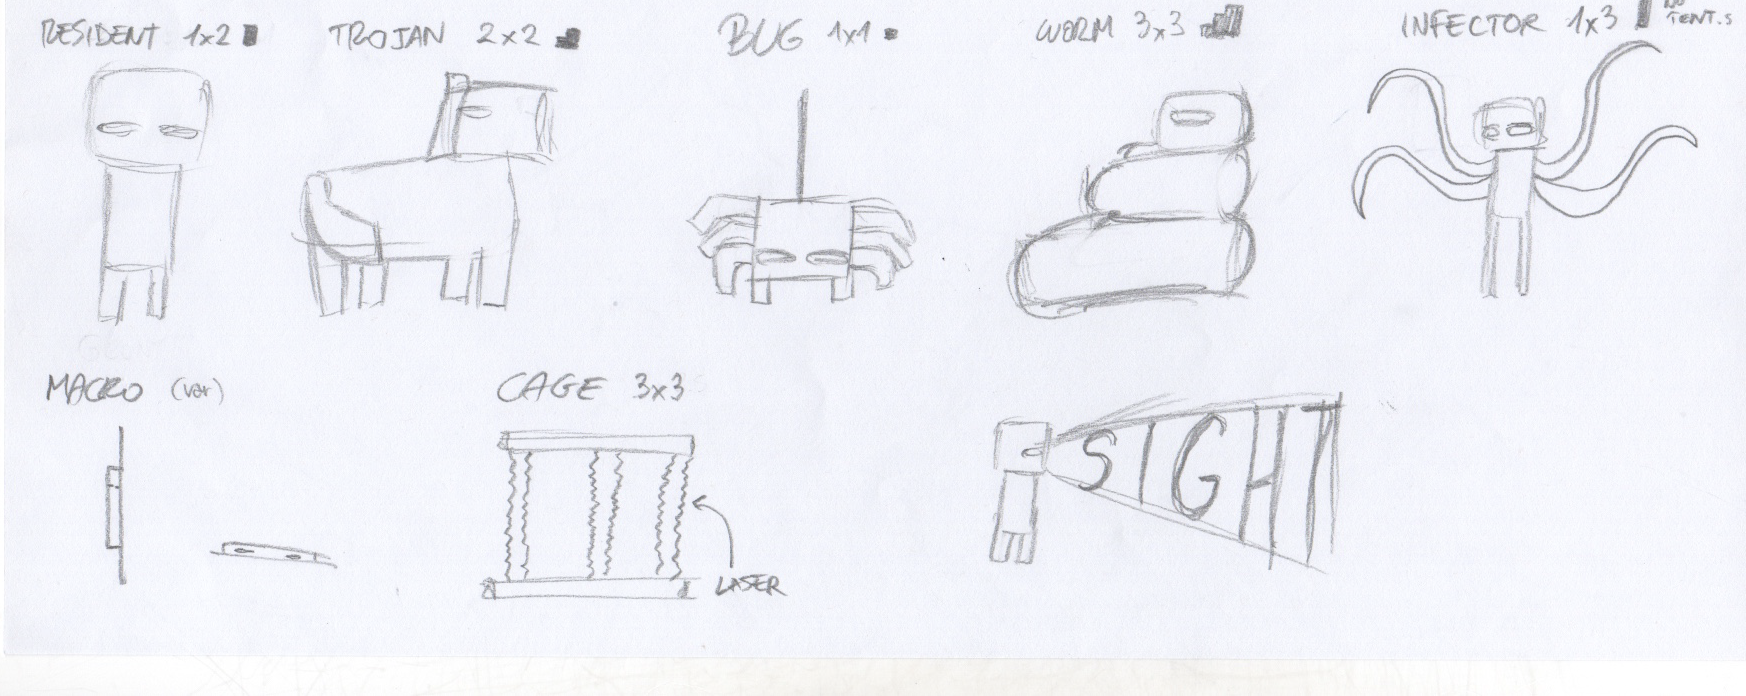
\includegraphics[width=0.5\textwidth]{images/Enemy}
\end{figure}
	\begin{figure}[H]
	\centering
	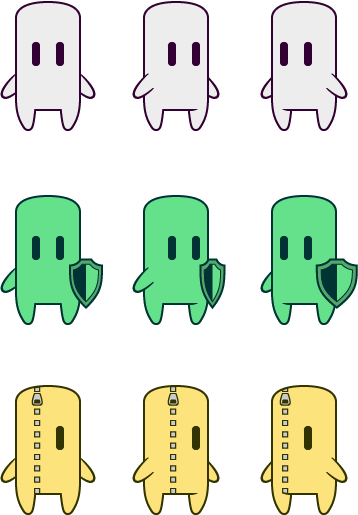
\includegraphics[width=0.3\textwidth]{images/Bits}
\end{figure}


\chapter{Sound Overview}
The soundtrack for \textit{Bit&Byte} takes inspiration from electronic music, particularly on the “trance” and “chill” side, to make the player feel like they are in a virtual world.
The sound effects are mostly simple and monophonic, reminescent of old-school arcade games.\\

\end{document}
